\documentclass[11pt]{article}
\usepackage{listings}
\usepackage{xcolor}
\usepackage{graphicx}
\usepackage[english]{babel}
\usepackage[utf8]{inputenc}
\usepackage{fancyhdr}
\usepackage[firstpage=true]{background}
\usepackage{multicol}
\usepackage{tikz}
\usepackage{subcaption}

\pagestyle{fancy}
\fancyhf{}
\rhead{Tarea 1 - \LaTeX{}}
\rfoot{Page \thepage}
\graphicspath{ {images/} }
\lstset
{
    language=[LaTeX]TeX,
    breaklines=true,
    basicstyle=\tt\scriptsize,
    keywordstyle=\color{blue},
    identifierstyle=\color{magenta},
}
\backgroundsetup{
contents={
\includegraphics{latex.png}},
angle=0,
scale=0.5,
color=black,
opacity=0.2
}

\title{\textbf{Tarea 1 - \LaTeX{}}}
\author{Ariel Herrera Fernandez\\Jorge Sibaja Sandi\\Saul Zamora Castro}
\date{}
\begin{document}

\maketitle

\newpage

\tableofcontents

\newpage

\section{Datos historicos}
\LaTeX{} es un sistema de composicion de texto, orientado a la creacion de documentos que presentan una alta calidad tipografica. Dadas sus caracteristicas y posibilidades, es usado particularmente en la generacion de articulos y libros cientificos que incluyen entre otas cosas, expresiones matematicas.

El sistema esta conformado por un gran conjunto de macros de TeX, escrito por Leslie Lamport en 1984 con la intencion de facilitar la composicion tipografica de TeX, que fue creado por Donald Knuth.

El ser de codigo abierto permite que muchos de sus usuarios realicen nuevas utilidades que extiendan las capacidades del sistema; las cuales no siempre tienen la misma intencion con la que \LaTeX{} fue creado. Para solucionar este problema, en 1989 Lamport y otros desarrolladores iniciaron lo que se conoce como el `Proyecto LaTeX3'. En 1993 se anuncio una reestandarizacion completa de \LaTeX{} mediante una nueva versio que incluyera la mayor parte de las extensiones adicionales para dar uniformmidad al conjunto y evitar la fragmentacion entre versiones incompatibles.

Una nueva version del sistema sale al publico cada año, aunque las diferencias entre una y otra suelen ser minimas, siempre estan bien documentadas.

\section{Importancia y usos academicos}
\LaTeX{} trabaja con una filosofia diferente de la de los procesadores de texto habituales (conocida como WYSIWYG `What You See Is What You Get' que significa `lo que ves es lo que obtienes'). Pero a diferencia de los otros procesadores, con \LaTeX{} el escritor puede dedicarse exclusivamente al contenido sin tener que preocuparse por los detalles de formato. Ademas de sus capacidades graficas para representar expresiones matematicas y formulas complicadas, notacion cientifica y musical, permite estructurar facilmente el documento, lo cual ofrece comodidad y lo hace util para articulos academicos y libros tecnicos.

La facilidad que presenta \LaTeX{} para insertar imagenes y graficas son la necesidad de estar pendiente de su ubicacion final en el documento (cosa que si hay que tener presente en los procesadores de texto mas habituales como Microsoft Word) es uno de los aspectos que lo hacen preferido por estudiantes para documentos como tesis.

Los documentos generados por \LaTeX{} son de muy alta calidad, especialmente cuando hay formulas matematicas involucradas. Otro factor que hace ventajoso a \LaTeX{} sobre otros procesadores de texto, es que no depende de ninguna plataforma para funcionar; asi como puede ser usado en Windows, puede ser utilizado en Linux o Mac OS.

\section{Uso de estructuras}

\subsection{Lo basico}

El siguiente codigo ejemplifica la creacion de titulos de documentos, autores, tablas de contenidos, secciones, parrafos y formulas matematicas.

\begin{lstlisting}
\documentclass{article}

\title{My first \LaTeX\ document}
\author{You!}

\begin{document}
	\maketitle
	\tableofcontents

	\section{My first Section}
	\label{firstSection}

	This is my first section!

	LaTeX is great in setting formulas 
	\\like in example $c = \sqrt{a^2 + b^2}$

	\section{My second Section}

	Even referencing other sections is very easy.
	\\See section~\ref{firstSection}.
\end{document}
\end{lstlisting}

Lo cual genera un documento como el de la siguiente figura.

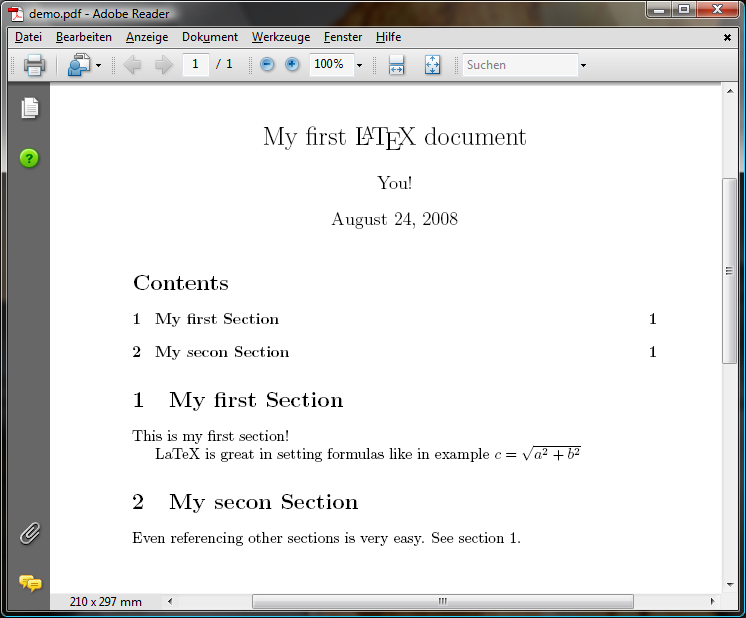
\includegraphics[width=0.9\textwidth]{ejemplo1.png}

\subsection{Como agregar efectos al texto}
Para agregar efectos al texto, tales como color o cursiva, se usa un snippet similar al siguiente:

\begin{lstlisting}
\emph{some black text, \color{red} followed by a red fragment}, going black again.
\end{lstlisting}

Lo cual genera un texto asi:\\
\emph{some black text, \color{red} followed by a red fragment}, going black again.

\subsection{Como agregar subtitulos}
Para agregar subtitulos para una seccion, se agregan `subsecciones' de la siguiente forma:

\begin{lstlisting}
\subsection{Estructuras basicas}
\end{lstlisting}

El codigo anterior es el utilizado para generar el subtitulo de la seccion 4.1 de este reporte.

\subsection{Como agregar referencias}
El codigo a continuacion es el necesario para agregar referencias bibliograficas:

\begin{lstlisting}
\begin{thebibliography}{9}

\bibitem{lamport94}
  Leslie Lamport,
  \emph{\LaTeX: a document preparation system},
  Addison Wesley, Massachusetts,
  2nd edition,
  1994.

\end{thebibliography}
\end{lstlisting}

El codigo anterior genera referencias similares a las de este documento.

\subsection{Como agregar marcas de agua}
La marca de agua en la primera pagina fue generada con el siguiente snippet:

\begin{lstlisting}
\backgroundsetup{
contents={
\includegraphics{latex.png}},
angle=0,
scale=0.5,
color=black,
opacity=0.2
}
\end{lstlisting}

\subsection{Como agregar encabezados y pies de pagina}
Para generar encabezados y pies de pagina como los de este documento se utilizan las sigioentes librerias:

\begin{lstlisting}
\usepackage[english]{babel}
\usepackage[utf8]{inputenc}
\usepackage{fancyhdr}
\end{lstlisting}

Y para el contenido se usa el siguiente codigo:

\begin{lstlisting}
\pagestyle{fancy}
\fancyhf{}
\rhead{Tarea 1 - \LaTeX{}}
\rfoot{Page \thepage}
\end{lstlisting}

\subsection{Como agregar columnas}
El siguiente codigo es un ejemplo de como crear un documento con columnas:

\begin{lstlisting}
\usepackage{multicol}
 
\begin{document}
\begin{multicols}{3}
[
\section{First Section}
All human things are subject to decay. And when fate summons, Monarchs must obey.
]
Hello, here is some text without a meaning.  This text should show what 
a printed text will look like at this place.
If you read this text, you will get no information.  Really?  Is there 
no information?  Is there...
\end{multicols}
\end{lstlisting}

El codigo anterior genera un texto de la siguiente forma:

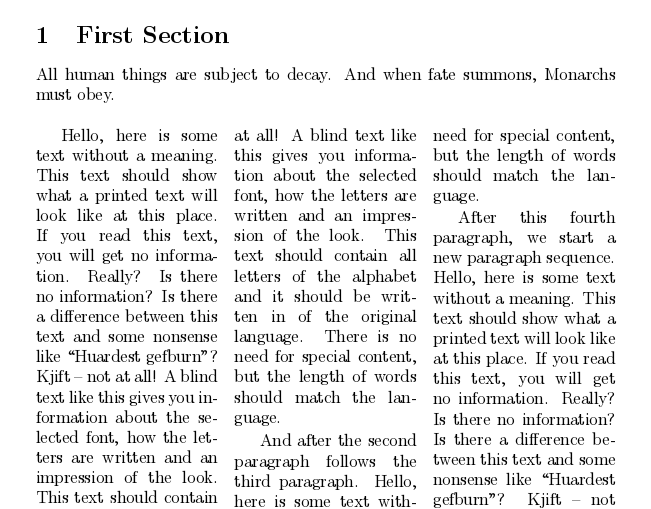
\includegraphics[width=0.9\textwidth]{ejemplo2.png}

\section{Como crear tablas}

Para crear tablas, se usa un codigo como el siguiente:

\begin{lstlisting}
\begin{table}[]
\centering
\caption{My caption}
\label{my-label}
\begin{tabular}{lllll}
 1 2 3 4 5  \\
 a b c d e  \\
 6 7 8 9 0  \\
 f g h i j 
\end{tabular}
\end{table}
\end{lstlisting}

El cual genera una tabla como la siguiente:

\begin{table}[]
\centering
\caption{My caption}
\label{my-label}
\begin{tabular}{lllll}
 1 2 3 4 5  \\
 a b c d e  \\
 6 7 8 9 0  \\
 f g h i j 
\end{tabular}
\end{table}

\section{Como crear graficos}

Las posibilidades al crear graficos en LaTeX son muchas, el siguiente es un ejemplo simple de como generar un grafico circular:

\begin{lstlisting}
\usepackage{tikz}
\begin{document}
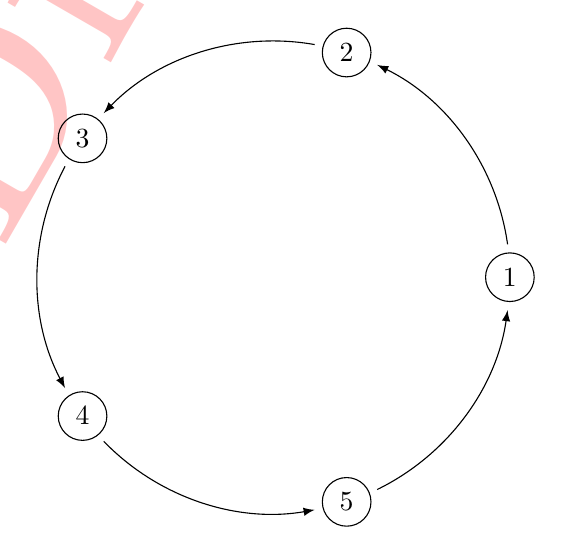
\begin{tikzpicture}

\def \n {5}
\def \radius {3cm}
\def \margin {8} % margin in angles, depends on the radius

\foreach \s in {1,...,\n}
{
  \node[draw, circle] at ({360/\n * (\s - 1)}:\radius) {$\s$};
  \draw[->, >=latex] ({360/\n * (\s - 1)+\margin}:\radius) 
    arc ({360/\n * (\s - 1)+\margin}:{360/\n * (\s)-\margin}:\radius);
}
\end{tikzpicture}
\end{document}
\end{lstlisting}

El cual genera un grafico como el siguiente:


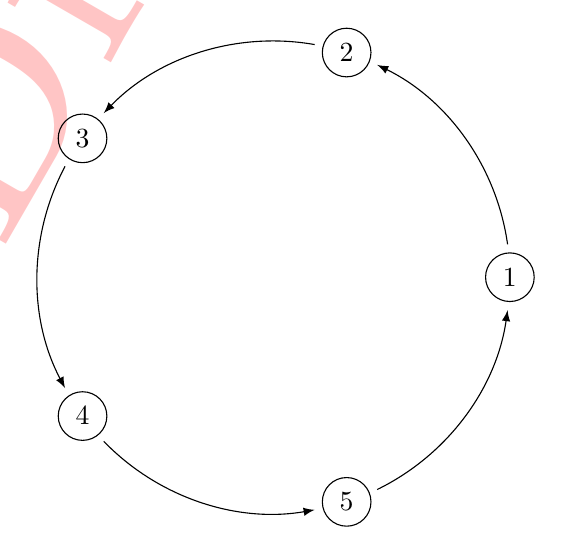
\begin{tikzpicture}

\def \n {5}
\def \radius {3cm}
\def \margin {8} % margin in angles, depends on the radius

\foreach \s in {1,...,\n}
{
  \node[draw, circle] at ({360/\n * (\s - 1)}:\radius) {$\s$};
  \draw[->, >=latex] ({360/\n * (\s - 1)+\margin}:\radius) 
    arc ({360/\n * (\s - 1)+\margin}:{360/\n * (\s)-\margin}:\radius);
}
\end{tikzpicture}


\section{Como agregar imagenes}
Para insertar imagenes se usa el siguiente codigo:

\begin{lstlisting}
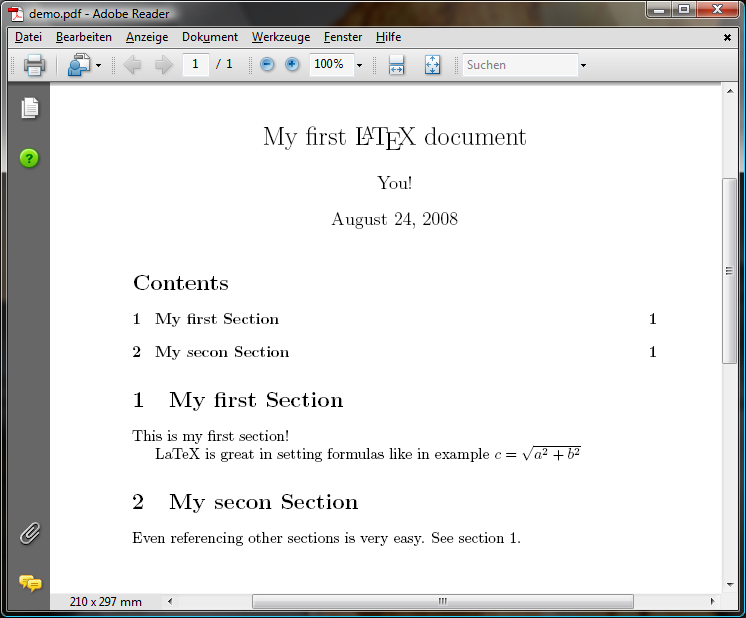
\includegraphics[width=0.9\textwidth]{ejemplo1.png}
\end{lstlisting}

Este codigo particular fue el utilizado para insertar la imagen en la seccion 4.1.

\section{Como agregar minipages}
Para insertar figuras al lado de figuras, tambien conocidas como \emph{minipages}, se utiliza un codigo similar a esto:

\begin{lstlisting}
\begin{figure}[h]
 
\begin{subfigure}{0.5\textwidth}
\includegraphics[width=0.9\linewidth, height=5cm]{lion-logo} 
\caption{Caption1}
\label{fig:subim1}
\end{subfigure}
\begin{subfigure}{0.5\textwidth}
\includegraphics[width=0.9\linewidth, height=5cm]{mesh}
\caption{Caption 2}
\label{fig:subim2}
\end{subfigure}
 
\caption{Caption for this figure with two images}
\label{fig:image2}
\end{figure}
\end{lstlisting}

Para utilizar el ambiente \emph{subfigure}, es necesario incluir el siguiente paquete:

\begin{lstlisting}
\usepackage{subcaption}
\end{lstlisting}

\begin{figure}[h]
 
\begin{subfigure}{0.5\textwidth}
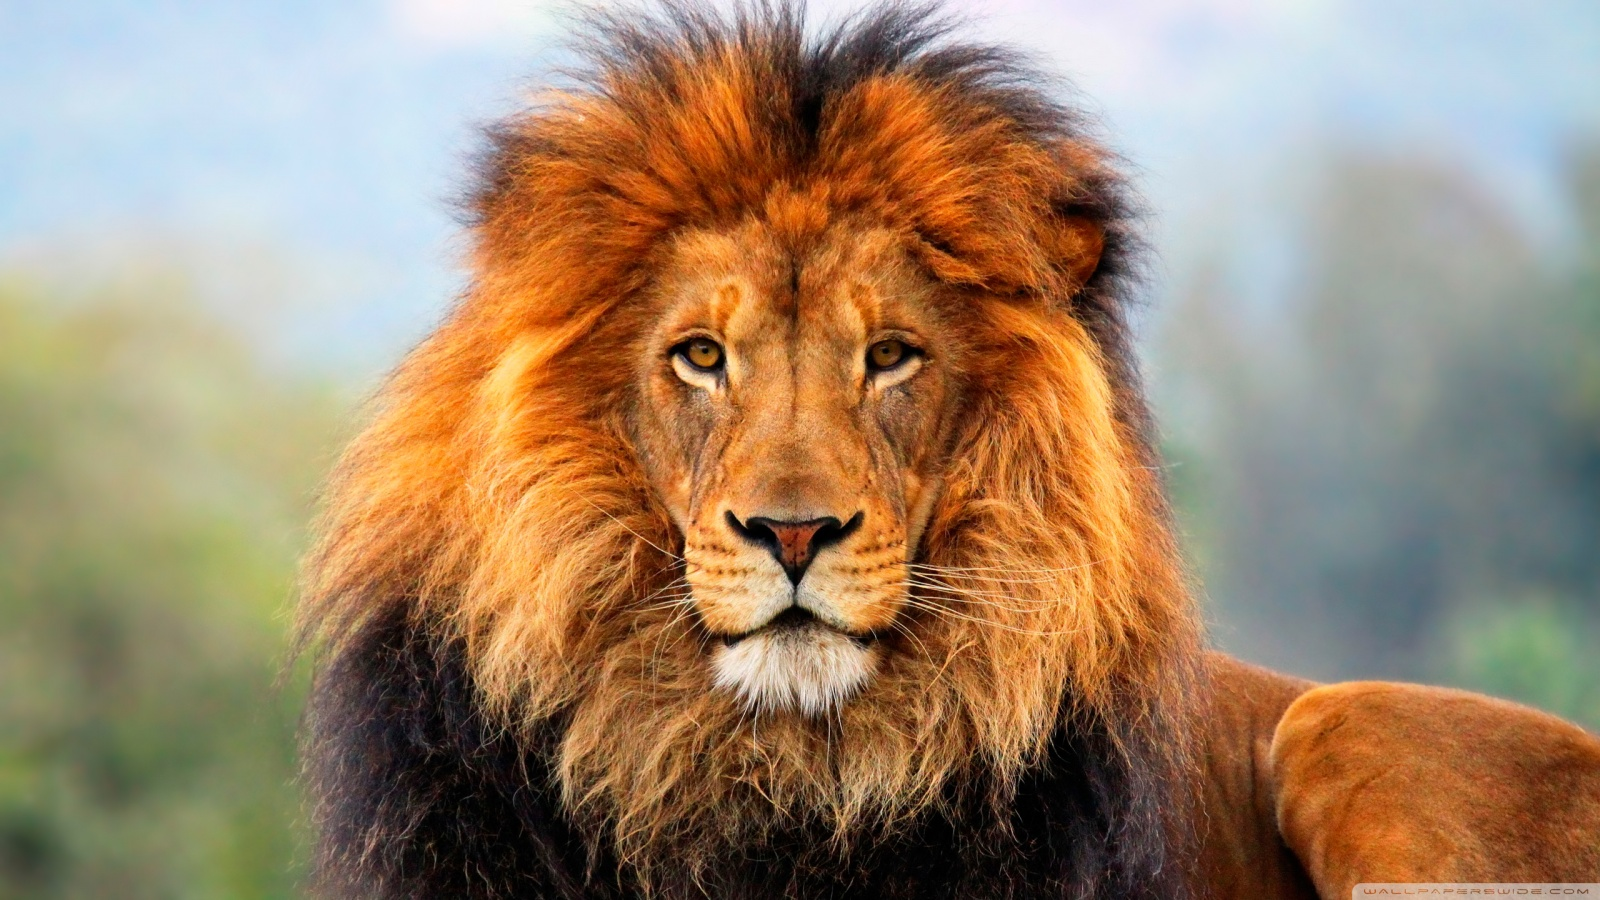
\includegraphics[width=0.9\linewidth, height=5cm]{lion} 
\caption{This is a Lion}
\label{fig:subim1}
\end{subfigure}
\begin{subfigure}{0.5\textwidth}

\includegraphics[width=0.9\linewidth, height=5cm]{tiger}
\caption{This is a Tiger}
\label{fig:subim2}
\end{subfigure}
 
\caption{Ejemplo de dos imagenes lado a lado}
\label{fig:image2}
\end{figure}
\newpage

\begin{thebibliography}{99}
\bibitem{TeXnicCenter} TeXnicCenter, \emph{About \LaTeX{}}, http://www.texniccenter.org/about/about-LaTeX
\bibitem{LaTeX} \LaTeX{}, Wikipedia, https://es.wikipedia.org/wiki/LaTeX
\bibitem{ShareLaTeX} ShareLaTeX Documentation, https://es.sharelatex.com/learn
\bibitem{LaTeX/Colors} \LaTeX{}/Colors, https://en.wikibooks.org/wiki/LaTeX/Colors
\end{thebibliography}
\end{document}